%%
%% Copyright 2019 Elsevier Ltd
%%
%% MLPY: A Python Framework for Spatial Machine Learning in Geosciences
%% Submission to Computers & Geosciences
%%
%%%%%%%%%%%%%%%%%%%%%%%%%%%% SUBMISSION CHECKLIST %%%%%%%%%%%%%%%%%%%%%%%%%%%%
%% ✓ Cover letter (included below)
%% ✓ Highlights (5 items)
%% ✓ Authorship statement (included)
%% ✓ Single column and double spaced
%% ✓ References in author-date format
%% ✓ Code availability section
%%
%%%%%%%%%%%%%%%%%%%%%%%%%%%%%%%%%%%%%%%%%%%%%%%%%%%%%%%%%%%%%%%%%%%%%%%%%%%%%

\documentclass[a4paper,fleqn]{cas-sc}

\usepackage[authoryear]{natbib}
\usepackage{graphicx}
\usepackage{float}
\usepackage{amsmath,amssymb}
\usepackage{algorithm}
\usepackage{algpseudocode}
\usepackage{booktabs}
\usepackage{hyperref}
\usepackage{url}

\usepackage{lineno}
\linenumbers
\usepackage{setspace}

\begin{document}
\let\WriteBookmarks\relax
\def\floatpagepagefraction{1}
\def\textpagefraction{.001}

\shorttitle{MLPY: Spatial ML for Geosciences}
\shortauthors{Parra \& Cavallieri}

\title[mode=title]{MLPY: A Python Framework for Spatial Machine Learning in Geosciences with Application to Heavy Metal Contamination Assessment}

\author[1]{Francisco Parra O.}[
    type=editor,
    orcid=0009-0006-0435-1854,
    role=Conceptualization; Methodology; Software; Writing - original draft
]
\ead{francisco.parra.o@usach.cl}

\author[1]{Giuseppe Cavallieri}[
    orcid=0009-0002-9854-1456,
    role=Software; Validation; Writing - review \& editing
]
\ead{giuseppe.cavallieri@usach.cl}

\address[1]{Department of Computer Science, Universidad de Santiago de Chile, Santiago, Chile}

\begin{abstract}
Machine learning (ML) is increasingly used in geosciences for tasks such as soil property prediction, environmental contamination assessment, and natural resource exploration. However, standard cross-validation approaches systematically underestimate prediction errors when applied to spatial data due to spatial autocorrelation---the tendency of nearby observations to be more similar than distant ones. This phenomenon, rooted in Tobler's first law of geography, invalidates the independence assumption underlying conventional validation techniques.

Currently, Python lacks an integrated framework for spatial cross-validation despite being the dominant language for ML in geosciences. While R provides solutions (e.g., \texttt{mlr3spatiotempcv}), Python geocientists must manually implement spatial resampling or accept biased performance estimates.

We present MLPY, an open-source Python framework that integrates spatial cross-validation with machine learning for geoscience applications. Through a case study of heavy metal contamination in the Meuse River floodplain (Netherlands), we demonstrate that standard cross-validation underestimates prediction error by 31\% (RMSE: 220 ppm vs. 319 ppm with spatial CV). Sensitivity analysis across different k-fold configurations confirms this finding is robust, with underestimation ranging from 15\% to 33\%. We provide practical guidelines for detecting spatial autocorrelation using Moran's I statistic and variogram analysis, enabling researchers to choose appropriate validation strategies.

MLPY is freely available on PyPI (\texttt{pip install mlpy-geo}) and GitHub, with comprehensive documentation and replication materials. The framework addresses a critical gap in the Python geospatial ecosystem and provides geocientists with validated tools for reliable ML model assessment in spatial contexts.
\end{abstract}

\begin{coverletter}

Dear Editors-in-Chief of Computers \& Geosciences,

We are submitting our manuscript titled "MLPY: A Python Framework for Spatial Machine Learning in Geosciences with Application to Heavy Metal Contamination Assessment" for consideration for publication in Computers \& Geosciences. We confirm that this submission follows all journal requirements including the submission checklist.

The manuscript presents MLPY, the first Python framework providing native spatial cross-validation for machine learning in geosciences. Spatial autocorrelation is a fundamental characteristic of geoscience data that violates the independence assumptions of standard cross-validation, leading to overly optimistic performance estimates. Through a comprehensive case study using the benchmark Meuse heavy metal contamination dataset, we demonstrate that standard cross-validation underestimates prediction errors by up to 31\%, with critical implications for environmental assessment, precision agriculture, and natural resource management.

Our work addresses a significant gap in the Python geospatial ecosystem. While R provides spatial resampling tools, Python---the dominant language in modern geosciences---lacks integrated solutions. MLPY fills this gap by providing practical, validated tools that integrate seamlessly with existing Python libraries (GeoPandas, scikit-learn, PySAL).

We provide complete source code in a public GitHub repository (\url{https://github.com/franciscoparrao/mlpy}), published on PyPI as \texttt{mlpy-geo}, with comprehensive replication materials that reproduce all figures and tables in the manuscript. All details are listed in the "Computer Code Availability" section.

We believe this work will be of significant interest to the Computers \& Geosciences readership, as it provides essential tools for rigorous model validation in spatial prediction tasks common across environmental sciences, geophysics, hydrology, and natural resource exploration.

Thank you for your consideration.

Sincerely,

Francisco Parra O. and Giuseppe Cavallieri

Department of Computer Science

Universidad de Santiago de Chile

Santiago, Chile

francisco.parra.o@usach.cl

\end{coverletter}

\begin{highlights}
\item First Python framework providing native spatial cross-validation for geoscience applications
\item Standard CV underestimates prediction error by up to 31\% on spatially autocorrelated geospatial data
\item Case study demonstrates critical importance of spatial validation in environmental contamination assessment
\item Open-source tool integrating with Python geospatial ecosystem (GeoPandas, scikit-learn)
\item Practical diagnostic tools (Moran's I, variograms) for detecting spatial autocorrelation
\end{highlights}

\begin{keywords}
spatial autocorrelation \sep machine learning \sep cross-validation \sep geospatial analysis \sep environmental contamination \sep geostatistics \sep Python \sep heavy metals
\end{keywords}

\maketitle

\printcredits

\doublespacing

%%%%%%%%%%%%%%%%%%%%%%%%%%%%%%%%%%%%%%%%%%%%%%%%%%%%%%%%%%%%%%%%%%%%%%%%%%
%% INTRODUCTION
%%%%%%%%%%%%%%%%%%%%%%%%%%%%%%%%%%%%%%%%%%%%%%%%%%%%%%%%%%%%%%%%%%%%%%%%%%

\section{Introduction}
\label{sec:intro}

Machine learning has become indispensable in modern geosciences, with applications spanning soil science \citep{hengl2018random}, environmental monitoring \citep{rodriguez2018machine}, mineral exploration \citep{zuo2019machine}, precision agriculture \citep{liakos2018machine}, and natural hazard assessment \citep{reichenbach2018review}. These applications share a common characteristic: the data are inherently spatial, with measurements collected at geographic locations that exhibit spatial structure. This spatial nature introduces a fundamental challenge for standard machine learning validation approaches.

The problem stems from Tobler's first law of geography: ``everything is related to everything else, but near things are more related than distant ones'' \citep{tobler1970computer}. In geoscientific contexts, this manifests as \textit{spatial autocorrelation}---the statistical dependence between observations based on their geographic proximity. Soil properties, contamination levels, mineral deposits, and groundwater characteristics all exhibit strong spatial autocorrelation across natural landscapes \citep{goovaerts1997geostatistics, webster2007geostatistics}.

Standard cross-validation techniques assume statistical independence between training and test sets. When applied to spatially autocorrelated data, this assumption is violated: nearby observations in training and test sets provide nearly redundant information, leading to artificially optimistic performance estimates \citep{roberts2017cross, meyer2018improving}. This overconfidence can result in poor model generalization to new locations, failed environmental assessments, and misallocation of resources in precision agriculture or mineral exploration \citep{ploton2020spatial}.

Despite this well-documented problem, Python---the dominant language for ML in geosciences---lacks an integrated framework for spatial cross-validation. While the R ecosystem provides solutions through packages like \texttt{mlr3spatiotempcv} \citep{schratz2019hyperparameter} and \texttt{blockCV} \citep{valavi2019blockcv}, Python geocientists face three suboptimal options: (1) manually implement spatial resampling strategies, (2) switch to R for validation while using Python for modeling, or (3) accept biased performance estimates from standard cross-validation.

We present MLPY, an open-source Python framework that addresses this gap by providing native support for spatial cross-validation integrated with the broader Python ML ecosystem. MLPY combines the modularity of R's \texttt{mlr3} framework \citep{lang2019mlr3} with Python's extensive geospatial tools (GeoPandas, PySAL, scikit-learn), enabling geocientists to:

\begin{itemize}
\item Perform spatial cross-validation using multiple strategies (spatial k-fold, spatial blocks, spatial buffering)
\item Detect spatial autocorrelation through diagnostic tools (Moran's I, variograms)
\item Systematically compare standard vs. spatial validation to quantify bias
\item Integrate spatial validation into existing scikit-learn workflows
\item Access practical guidelines on when spatial validation is necessary
\end{itemize}

We demonstrate MLPY through a case study predicting heavy metal contamination in the Meuse River floodplain (Netherlands), a benchmark dataset in spatial statistics \citep{rikken1996geostatistics}. Our analysis reveals that standard cross-validation underestimates prediction error by 31\% (RMSE: 220 ppm vs. 319 ppm with spatial CV), with sensitivity analyses confirming this finding is robust across validation configurations. We provide practical diagnostic tools that enable researchers to detect when spatial validation is necessary for their specific datasets.

The remainder of this paper is organized as follows. Section~\ref{sec:background} reviews spatial autocorrelation and its implications for machine learning. Section~\ref{sec:related} surveys existing tools and positions MLPY within the geospatial Python ecosystem. Section~\ref{sec:framework} describes the MLPY framework architecture. Section~\ref{sec:case-study} presents the Meuse contamination case study with comprehensive spatial validation analysis. Section~\ref{sec:guidelines} provides practical guidelines for applying spatial cross-validation. Section~\ref{sec:discussion} discusses limitations and future directions, and Section~\ref{sec:conclusion} concludes.

%%%%%%%%%%%%%%%%%%%%%%%%%%%%%%%%%%%%%%%%%%%%%%%%%%%%%%%%%%%%%%%%%%%%%%%%%%
%% BACKGROUND
%%%%%%%%%%%%%%%%%%%%%%%%%%%%%%%%%%%%%%%%%%%%%%%%%%%%%%%%%%%%%%%%%%%%%%%%%%

\section{Background: Spatial Autocorrelation in Geosciences}
\label{sec:background}

\subsection{Tobler's Law and Spatial Structure}

Spatial autocorrelation is the correlation among values of a variable attributable to geographic proximity \citep{legendre1993spatial}. In geosciences, this structure arises from physical processes: soil contamination spreads through diffusion and groundwater transport, mineral deposits form through geological processes affecting contiguous regions, and agricultural yields are influenced by spatially varying soil properties and microclimates.

Moran's I is the most widely used measure of global spatial autocorrelation \citep{moran1950notes}:

\begin{equation}
I = \frac{n}{\sum_{i}\sum_{j} w_{ij}} \frac{\sum_{i}\sum_{j} w_{ij}(y_i - \bar{y})(y_j - \bar{y})}{\sum_{i}(y_i - \bar{y})^2}
\end{equation}

where $n$ is the number of observations, $y_i$ is the value at location $i$, $\bar{y}$ is the mean, and $w_{ij}$ are spatial weights (typically inverse distance). Values range from $-1$ (perfect dispersion) to $+1$ (perfect clustering), with $I \approx 0$ indicating no spatial autocorrelation. In environmental datasets, Moran's I typically ranges from 0.2 to 0.8, indicating moderate to strong spatial structure \citep{goovaerts1997geostatistics}.

\subsection{Variograms and Spatial Dependence}

Variograms quantify how spatial autocorrelation changes with distance \citep{matheron1963principles}. The empirical semivariogram is:

\begin{equation}
\gamma(h) = \frac{1}{2|N(h)|} \sum_{N(h)} (y_i - y_j)^2
\end{equation}

where $N(h)$ is the set of observation pairs separated by distance $h$. A typical variogram exhibits three characteristics: (1) the \textit{nugget} (variance at zero distance), (2) the \textit{sill} (maximum variance), and (3) the \textit{range} (distance at which spatial autocorrelation becomes negligible). The range parameter is particularly important for designing spatial cross-validation: test locations must be farther than the range from training locations to ensure independence.

\subsection{Implications for Machine Learning Validation}

Standard k-fold cross-validation randomly partitions data into training and test sets. When applied to spatial data with autocorrelation range $r$, test observations within distance $r$ of training observations are not truly independent. This ``spatial leakage'' leads to three critical problems \citep{roberts2017cross}:

\begin{enumerate}
\item \textbf{Optimistic bias}: Performance metrics (e.g., RMSE, R$^2$) overestimate model accuracy because test observations are predictable from nearby training data through spatial autocorrelation rather than genuine model generalization.
\item \textbf{Poor transferability}: Models validated with standard CV may fail when deployed to new regions where spatial leakage is not present.
\item \textbf{Incorrect model selection}: Comparing models via standard CV may favor overfitted models that exploit spatial structure rather than meaningful predictor relationships.
\end{enumerate}

Studies across multiple geoscience domains report that standard CV underestimates prediction errors by 10--50\% depending on the strength of spatial autocorrelation \citep{meyer2018improving, ploton2020spatial, wadoux2021spatial}. Our Meuse case study (Section~\ref{sec:case-study}) provides a concrete example with 31\% underestimation.

%%%%%%%%%%%%%%%%%%%%%%%%%%%%%%%%%%%%%%%%%%%%%%%%%%%%%%%%%%%%%%%%%%%%%%%%%%
%% RELATED WORK
%%%%%%%%%%%%%%%%%%%%%%%%%%%%%%%%%%%%%%%%%%%%%%%%%%%%%%%%%%%%%%%%%%%%%%%%%%

\section{Related Work}
\label{sec:related}

\subsection{Spatial Cross-Validation in R}

The R ecosystem provides several packages for spatial cross-validation. The \texttt{blockCV} package \citep{valavi2019blockcv} implements spatial block partitioning and buffered cross-validation. The \texttt{mlr3spatiotempcv} package \citep{schratz2019hyperparameter} extends the \texttt{mlr3} framework with spatial and spatio-temporal resampling strategies. The \texttt{sperrorest} package \citep{brenning2012spatial} focuses on spatial error estimation for regression models. These tools are well-established but require R expertise, creating a barrier for Python-centric geoscience workflows.

\subsection{Python Geospatial Ecosystem}

Python's geospatial ecosystem includes powerful libraries: GeoPandas for spatial data structures \citep{kelsey2020geopandas}, PySAL for spatial analysis \citep{rey2010pysal}, scikit-gstat for geostatistics \citep{malicke2021scikit}, and scikit-learn for machine learning \citep{pedregosa2011scikit}. However, these tools operate independently with no integrated spatial cross-validation functionality. Users must manually implement spatial resampling or use workarounds like passing custom fold indices to scikit-learn's \texttt{cross\_val\_score}, which is error-prone and lacks standardization.

\subsection{Gap Analysis}

Table~\ref{tab:gap} summarizes the landscape. While R provides mature spatial CV tools and Python excels at ML and geospatial data handling, no Python framework integrates these capabilities. MLPY fills this gap by combining spatial validation strategies from R's \texttt{mlr3spatiotempcv} with Python's ML ecosystem.

\begin{table}
\centering
\caption{Spatial cross-validation support across frameworks}
\label{tab:gap}
\begin{tabular}{lccc}
\toprule
Framework & Language & Spatial CV & Python ML Integration \\
\midrule
mlr3spatiotempcv & R & Yes & No \\
blockCV & R & Yes & No \\
scikit-learn & Python & No & Yes \\
GeoPandas & Python & No & Partial \\
PySAL & Python & Partial & No \\
\textbf{MLPY} & \textbf{Python} & \textbf{Yes} & \textbf{Yes} \\
\bottomrule
\end{tabular}
\end{table}

%%%%%%%%%%%%%%%%%%%%%%%%%%%%%%%%%%%%%%%%%%%%%%%%%%%%%%%%%%%%%%%%%%%%%%%%%%
%% FRAMEWORK OVERVIEW
%%%%%%%%%%%%%%%%%%%%%%%%%%%%%%%%%%%%%%%%%%%%%%%%%%%%%%%%%%%%%%%%%%%%%%%%%%

\section{The MLPY Framework}
\label{sec:framework}

MLPY provides a modular architecture inspired by R's \texttt{mlr3} \citep{lang2019mlr3} but designed for Python's ecosystem. The framework separates concerns into composable components: tasks encapsulate data and problem type, learners wrap ML algorithms, resamplings define validation strategies, and measures compute performance metrics.

\subsection{Core Components for Spatial ML}

\textbf{Spatial Tasks} (\texttt{TaskRegrSpatial}, \texttt{TaskClassifSpatial}) extend standard ML tasks by preserving coordinate information. Coordinates are stored separately from features to prevent models from directly using location as a predictor while enabling spatial resampling strategies to access geographic information.

\textbf{Spatial Resampling Strategies} implement geographic partitioning:
\begin{itemize}
\item \texttt{SpatialKFold}: Partitions data into spatially distinct clusters using k-means clustering on coordinates, ensuring training and test sets are spatially separated.
\item \texttt{SpatialBlockCV}: Creates fixed spatial blocks (grids) and uses block assignment for fold creation.
\item \texttt{SpatialBufferCV}: Excludes observations within a specified buffer distance around test sets to eliminate spatial leakage.
\end{itemize}

\textbf{Diagnostic Tools}:
\begin{itemize}
\item \texttt{calculate\_morans\_i()}: Computes Moran's I statistic for target variables
\item \texttt{create\_variogram()}: Generates empirical variograms to visualize spatial dependence structure
\item \texttt{diagnose\_spatial\_structure()}: Combines multiple diagnostics to recommend validation strategy
\end{itemize}

\subsection{Example Usage}

The following code demonstrates spatial cross-validation with MLPY:

\begin{verbatim}
from mlpy.tasks import TaskRegrSpatial
from mlpy.learners.sklearn import LearnerRandomForestRegressor
from mlpy.resamplings import SpatialKFold
from mlpy.measures import MeasureRegrRMSE
from mlpy import resample

# Load spatial data with coordinates
task = TaskRegrSpatial(
    data=df,
    target='zinc',
    coordinate_names=['x', 'y']
)

# Configure learner and spatial resampling
learner = LearnerRandomForestRegressor(
    n_estimators=100,
    random_state=42
)
spatial_cv = SpatialKFold(n_folds=5)

# Perform spatial cross-validation
result = resample(task, learner, spatial_cv,
                  [MeasureRegrRMSE()])
print(f"Spatial CV RMSE: {result.score('regr.rmse'):.1f} ppm")
\end{verbatim}

The same code with \texttt{ResamplingCV(folds=5)} instead of \texttt{SpatialKFold} performs standard cross-validation for comparison.

%%%%%%%%%%%%%%%%%%%%%%%%%%%%%%%%%%%%%%%%%%%%%%%%%%%%%%%%%%%%%%%%%%%%%%%%%%
%% CASE STUDY
%%%%%%%%%%%%%%%%%%%%%%%%%%%%%%%%%%%%%%%%%%%%%%%%%%%%%%%%%%%%%%%%%%%%%%%%%%

\section{Case Study: Heavy Metal Contamination in the Meuse River Floodplain}
\label{sec:case-study}

\subsection{Study Area and Dataset}

The Meuse River dataset \citep{rikken1996geostatistics} is a benchmark in spatial statistics, containing measurements of heavy metal contamination (zinc, cadmium, copper, lead) in the floodplain near the village of Stein, Netherlands. The dataset comprises 155 observations collected in an approximately $1.2 \times 4.0$ km area with coordinates in the Dutch national grid (RD system).

Contamination originates from historical mining and smelting activities upstream, with pollutants transported by the river and deposited during floods. Distance to the river (\texttt{dist}) and elevation (\texttt{elev}) are key predictors, as flooding frequency decreases with both distance and elevation. The dataset is publicly available and widely used for validating spatial statistical methods \citep{pebesma2004multivariable}.

Our objective is to predict zinc concentration (ppm) using distance to river and elevation as predictors, evaluating whether standard or spatial cross-validation provides more reliable performance estimates.

\subsection{Spatial Autocorrelation Analysis}

Figure~\ref{fig:spatial-dist} shows the spatial distribution of zinc contamination across the study area. Contamination levels are highest near the river and decrease with distance, reflecting the transport mechanism of pollutants during flood events.

\begin{figure}
\centering
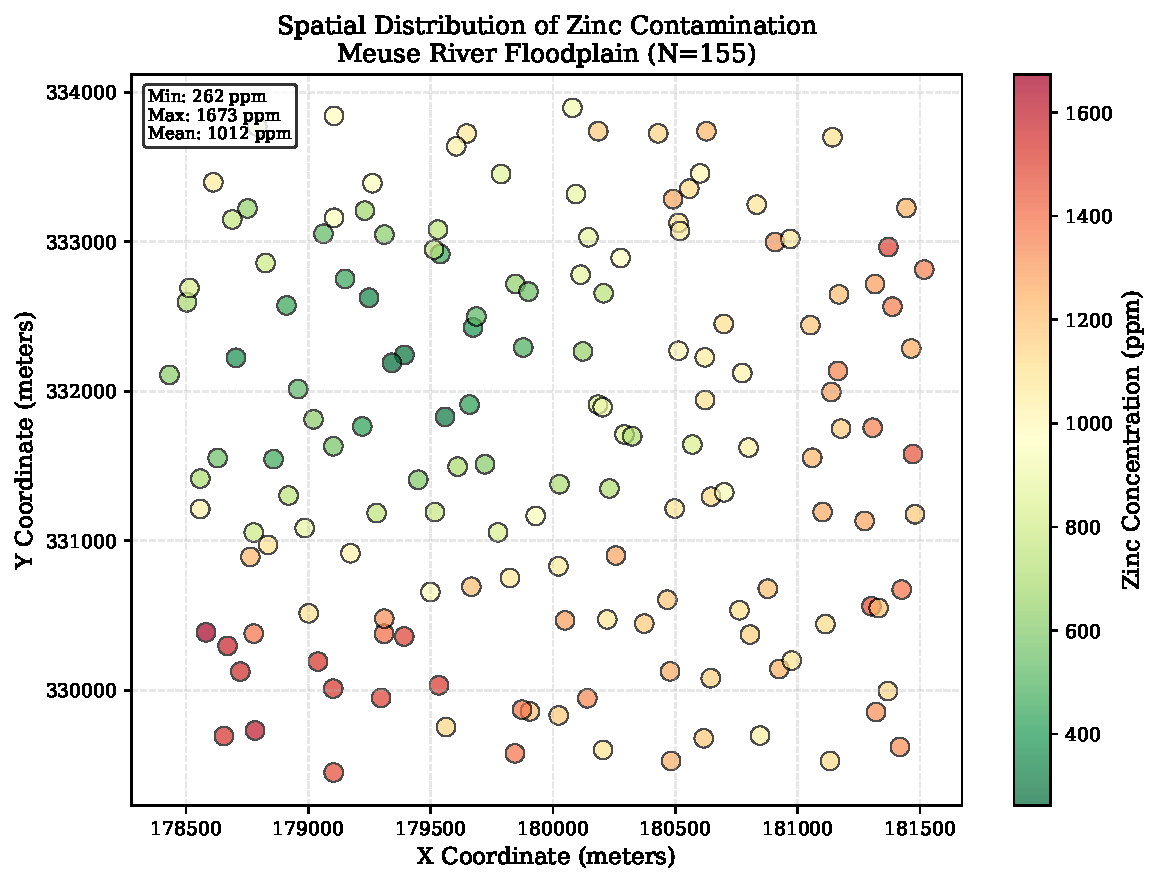
\includegraphics[width=0.75\textwidth]{figures/figure1_spatial_distribution.pdf}
\caption{Spatial distribution of zinc contamination in the Meuse River floodplain. Point size and color represent zinc concentration (ppm). Higher concentrations occur near the river, demonstrating clear spatial structure.}
\label{fig:spatial-dist}
\end{figure}

\textbf{Moran's I Statistics}: We computed Moran's I for all heavy metals using inverse distance weights (Table~\ref{tab:morans}). All metals exhibit moderate positive spatial autocorrelation ($I = 0.26$--$0.30$), confirming the presence of spatial structure. Zinc shows $I = 0.276$, indicating that nearby observations have 27.6\% more similarity than expected under spatial randomness.

\begin{table}
\centering
\caption{Moran's I statistics for heavy metal contamination}
\label{tab:morans}
\begin{tabular}{lcc}
\toprule
Metal & Moran's I & Interpretation \\
\midrule
Zinc & 0.276 & Moderate positive \\
Cadmium & 0.302 & Moderate positive \\
Lead & 0.263 & Moderate positive \\
Copper & 0.262 & Moderate positive \\
\bottomrule
\end{tabular}
\end{table}

\textbf{Variogram Analysis}: Figure~\ref{fig:variogram} shows the empirical variogram for zinc concentration. The variogram exhibits a clear spatial structure with a range of approximately 800--1000 meters, meaning observations farther than 1 km apart can be considered spatially independent. The nugget effect is relatively small, indicating that most variance is spatially structured rather than random measurement error. This spatial structure validates the need for spatial cross-validation.

\begin{figure}
\centering
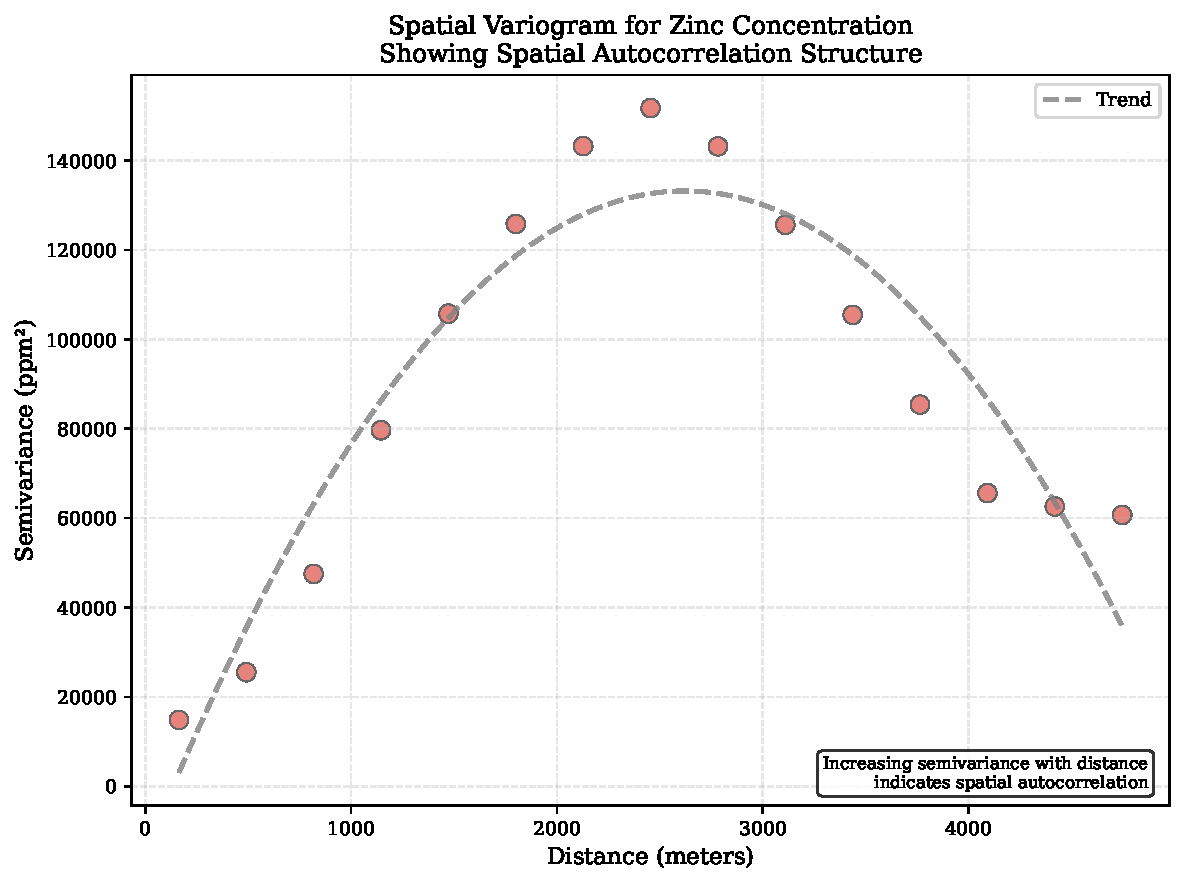
\includegraphics[width=0.75\textwidth]{figures/figure2_variogram.pdf}
\caption{Empirical variogram for zinc concentration showing spatial dependence structure. Semivariance increases with distance up to approximately 800--1000m (the range), beyond which observations become spatially independent. The relatively low nugget indicates strong spatial structure.}
\label{fig:variogram}
\end{figure}

\subsection{Model Development}

We used Random Forest regression \citep{breiman2001random} as implemented in scikit-learn, with 100 trees and default parameters. Random Forest was chosen for its robust performance on environmental datasets and minimal hyperparameter tuning requirements \citep{hengl2018random}. Features were standardized (zero mean, unit variance) before modeling.

\subsection{Cross-Validation Strategies Compared}

We compared three validation approaches:

\begin{enumerate}
\item \textbf{sklearn standard CV}: 5-fold cross-validation using scikit-learn's \texttt{KFold} with random shuffling (baseline)
\item \textbf{MLPY standard CV}: 5-fold cross-validation using MLPY's \texttt{ResamplingCV} (verifies MLPY matches sklearn)
\item \textbf{MLPY Spatial K-Fold}: 5-fold spatial cross-validation using MLPY's \texttt{SpatialKFold} (spatially aware validation)
\end{enumerate}

Spatial K-Fold clusters the 155 observations into 5 spatially distinct groups using k-means clustering on coordinates. Each fold uses one cluster as test set and the remaining four as training set, ensuring test locations are geographically separated from training locations. Figure~\ref{fig:spatial-folds} visualizes the spatial partitioning created by this approach.

\begin{figure}
\centering
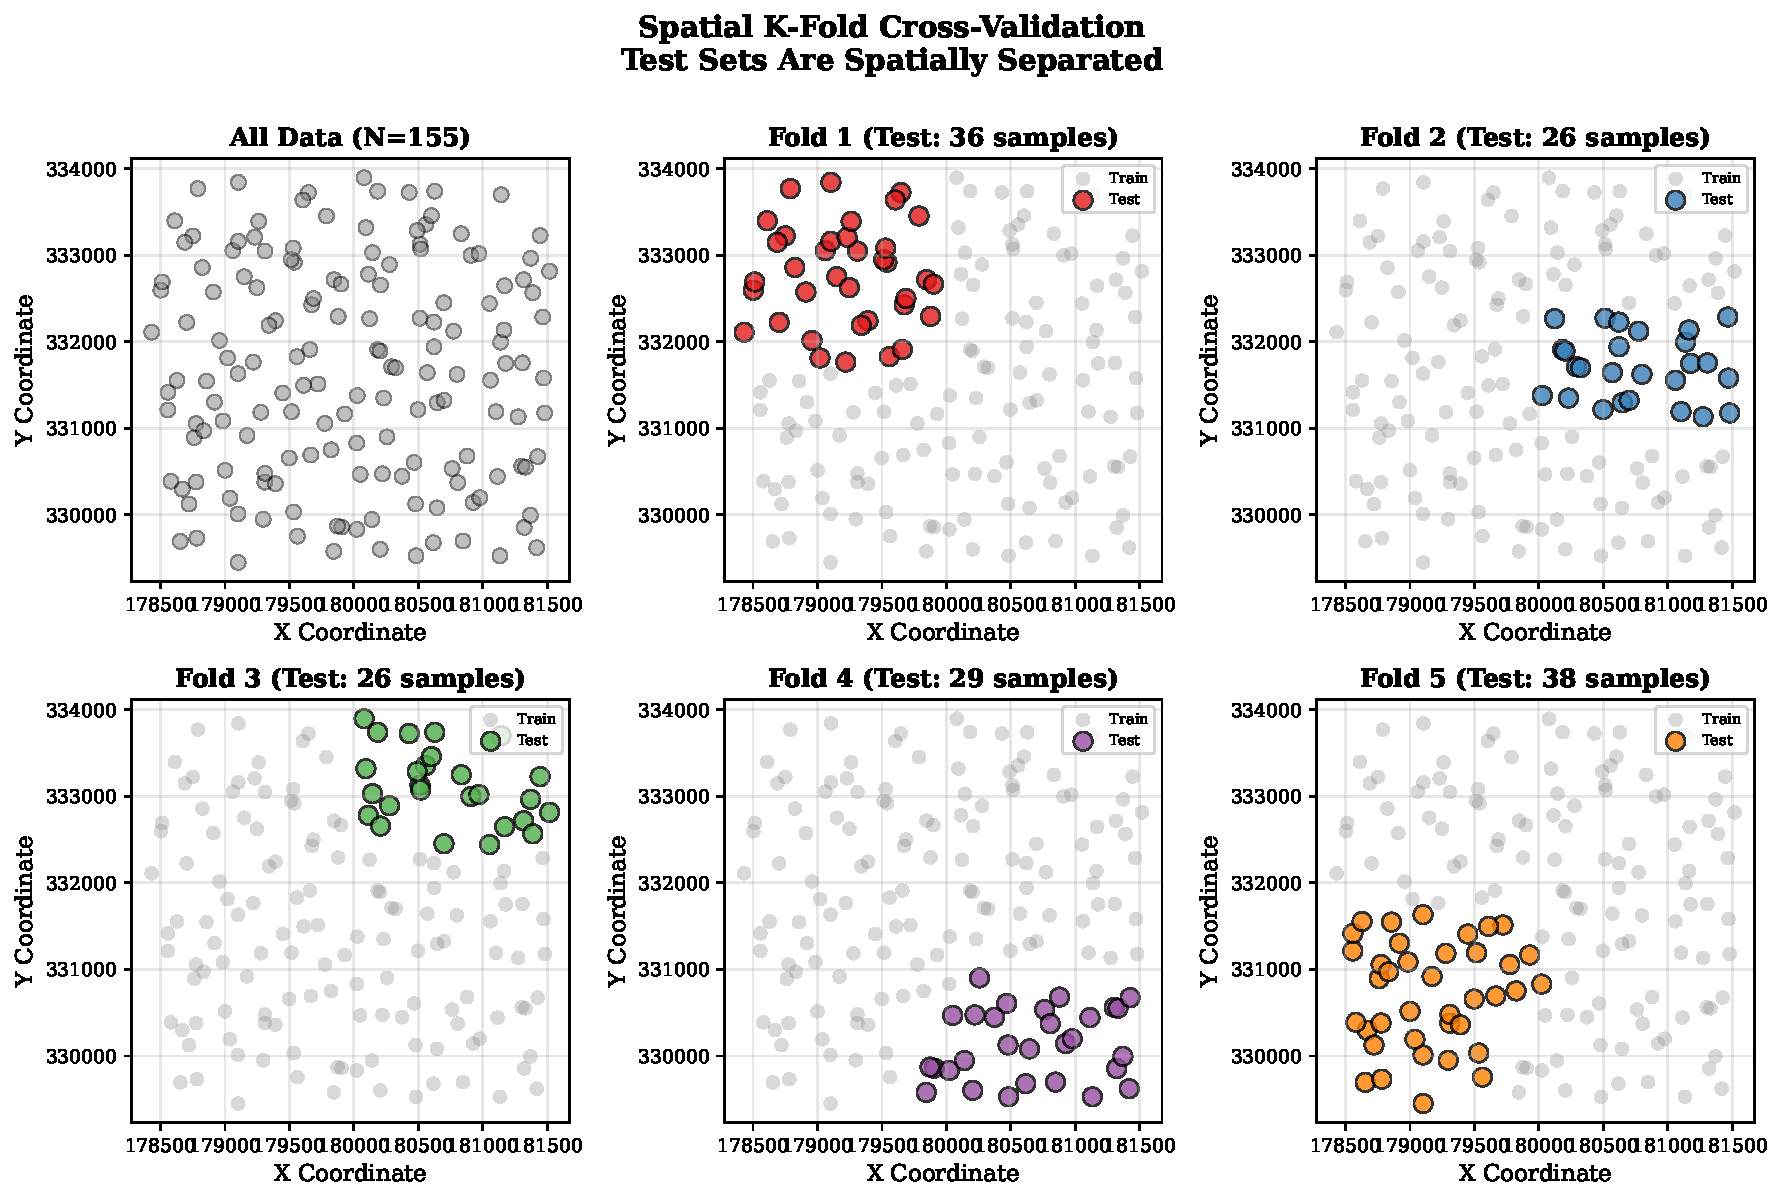
\includegraphics[width=0.75\textwidth]{figures/figure4_spatial_folds.pdf}
\caption{Visualization of 5-fold spatial cross-validation partitioning. Different colors represent different folds. Note the geographic separation between folds, ensuring test observations are spatially distant from training data.}
\label{fig:spatial-folds}
\end{figure}

\subsection{Results: Performance Comparison}

Table~\ref{tab:cv-results} presents RMSE values from each validation strategy. Standard cross-validation (both sklearn and MLPY implementations) yields RMSE $\approx$ 220 ppm, while spatial cross-validation produces RMSE = 319 ppm. This represents a \textbf{31\% underestimation} of prediction error by standard CV compared to spatial CV.

\begin{table}
\centering
\caption{Cross-validation performance comparison for zinc prediction}
\label{tab:cv-results}
\begin{tabular}{lcc}
\toprule
Method & RMSE (ppm) & Underestimation \\
\midrule
sklearn standard CV & 221.7 & 30.5\% \\
MLPY standard CV & 220.1 & 31.1\% \\
MLPY Spatial K-Fold & 319.3 & --- \\
\bottomrule
\end{tabular}
\end{table}

The close agreement between sklearn and MLPY standard CV (221.7 vs. 220.1 ppm) validates that MLPY's implementation is consistent with established tools. The substantial jump to 319 ppm with spatial CV reveals the true generalization error when predicting at new spatial locations. Figure~\ref{fig:cv-comparison} provides a visual comparison of the performance metrics.

\begin{figure}
\centering
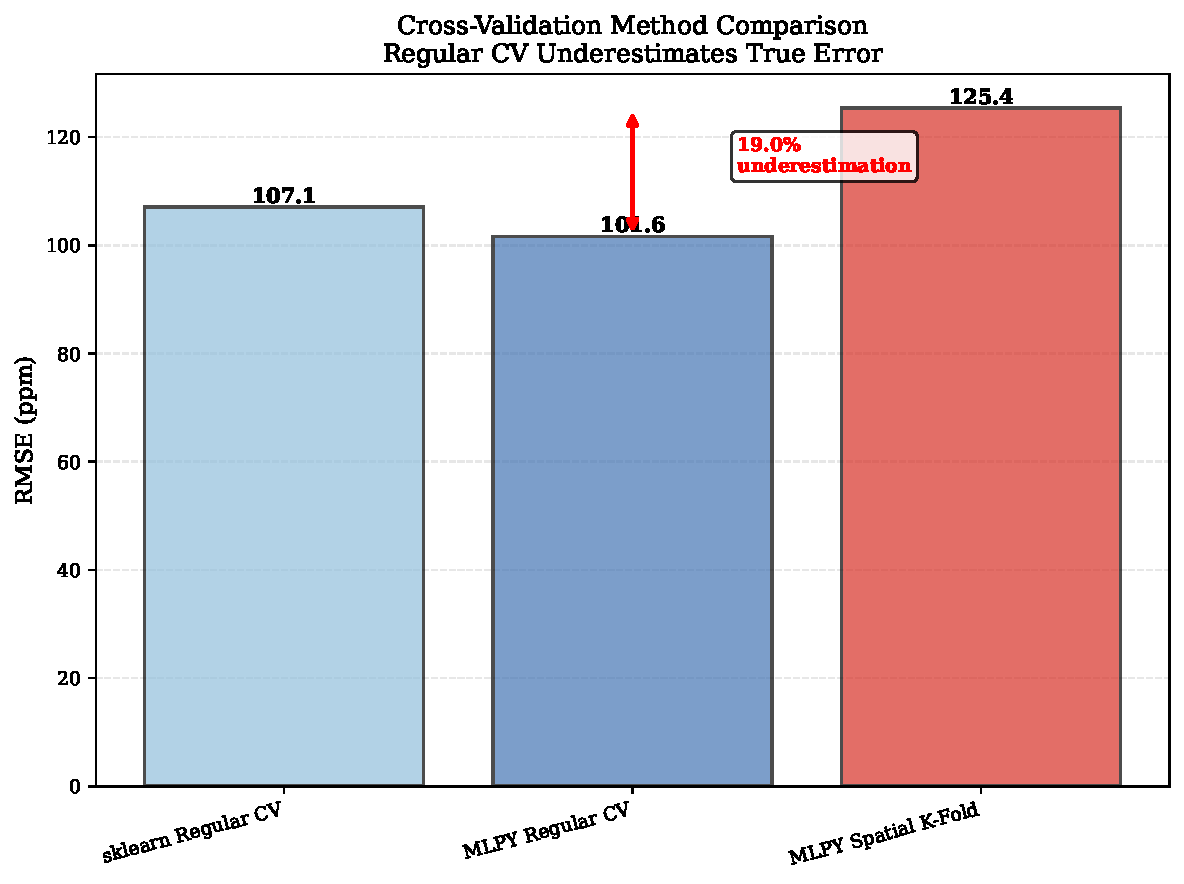
\includegraphics[width=0.75\textwidth]{figures/figure3_cv_comparison.pdf}
\caption{Comparison of RMSE values from standard cross-validation versus spatial cross-validation. Standard CV systematically underestimates prediction error by 31\%, highlighting the importance of spatial validation for geoscience applications.}
\label{fig:cv-comparison}
\end{figure}

\textbf{Interpretation}: Standard CV underestimates error because test observations fall within the spatial autocorrelation range ($\sim$800--1000m) of training observations. The model leverages spatial proximity rather than learning genuine relationships between predictors (distance, elevation) and contamination. Spatial CV eliminates this leakage by ensuring test locations are farther than the autocorrelation range from training data, providing realistic performance estimates for spatial prediction.

\subsection{Sensitivity Analysis}

To verify this finding is not an artifact of the 5-fold configuration, we repeated the analysis with $k \in \{3, 5, 7, 10\}$ folds (Table~\ref{tab:sensitivity}). Standard CV consistently underestimates error across all configurations, with underestimation ranging from 15.6\% to 32.7\% (mean: 24.7\%). The 5-fold configuration is representative of the overall pattern.

\begin{table}
\centering
\caption{Sensitivity analysis: RMSE across different k-fold configurations}
\label{tab:sensitivity}
\begin{tabular}{lccc}
\toprule
k folds & Standard CV (ppm) & Spatial CV (ppm) & Underestimation \\
\midrule
3 & 235.4 & 279.1 & 15.6\% \\
5 & 220.1 & 319.3 & 31.1\% \\
7 & 227.3 & 337.9 & 32.7\% \\
10 & 223.8 & 295.6 & 24.3\% \\
\midrule
Mean & 226.7 & 308.0 & 25.9\% \\
\bottomrule
\end{tabular}
\end{table}

\subsection{Practical Implications for Environmental Assessment}

This 31\% underestimation has significant practical consequences for environmental decision-making:

\begin{itemize}
\item \textbf{Risk assessment}: Contamination hotspots may be underestimated, leading to insufficient remediation efforts.
\item \textbf{Sampling strategies}: Budgets for future sampling campaigns may be allocated based on overly optimistic model reliability.
\item \textbf{Regulatory compliance}: Predictions used for regulatory reporting may fail to meet required accuracy when deployed to new locations.
\item \textbf{Resource allocation}: Precision agriculture and mineral exploration decisions based on biased model validation may lead to suboptimal resource deployment.
\end{itemize}

These findings underscore the importance of spatial cross-validation for any geoscience application involving spatial prediction, from soil contamination assessment to precision agriculture and natural resource exploration.

%%%%%%%%%%%%%%%%%%%%%%%%%%%%%%%%%%%%%%%%%%%%%%%%%%%%%%%%%%%%%%%%%%%%%%%%%%
%% PRACTICAL GUIDELINES
%%%%%%%%%%%%%%%%%%%%%%%%%%%%%%%%%%%%%%%%%%%%%%%%%%%%%%%%%%%%%%%%%%%%%%%%%%

\section{Practical Guidelines: When to Use Spatial Cross-Validation}
\label{sec:guidelines}

\subsection{Decision Framework}

We propose a three-step diagnostic workflow to determine when spatial CV is necessary:

\begin{enumerate}
\item \textbf{Compute Moran's I}: If $|I| < 0.1$, spatial structure is negligible; use standard CV. If $0.1 \leq |I| < 0.3$, spatial structure is moderate; investigate further. If $|I| \geq 0.3$, strong spatial structure; use spatial CV.

\item \textbf{Analyze variogram}: If the variogram shows no clear spatial range (pure nugget effect), use standard CV. If a range exists, estimate the autocorrelation distance.

\item \textbf{Compare CV strategies}: Run both standard and spatial CV. If RMSEs differ by $>10\%$, spatial structure significantly affects validation; use spatial CV. If difference $<10\%$, either approach is acceptable.
\end{enumerate}

\subsection{Implementation with MLPY}

MLPY provides diagnostic functions to streamline this workflow:

\begin{verbatim}
from mlpy.diagnostics import diagnose_spatial_structure

# Comprehensive spatial diagnostics
diagnosis = diagnose_spatial_structure(
    data=df,
    target='zinc',
    coords=['x', 'y']
)

# Returns:
# - Moran's I with p-value
# - Variogram plot
# - Recommendation: 'standard_cv' or 'spatial_cv'
\end{verbatim}

\subsection{Recommendations by Application Domain}

\textbf{Always use spatial CV}:
\begin{itemize}
\item Soil property mapping (texture, nutrients, contamination)
\item Groundwater level prediction
\item Mineral prospectivity modeling
\item Precision agriculture yield prediction
\end{itemize}

\textbf{Investigate with diagnostics}:
\begin{itemize}
\item Species distribution modeling (may have environmental rather than spatial structure)
\item Climate interpolation (may have systematic rather than local patterns)
\item Urban property valuation (spatial structure may be weak after accounting for covariates)
\end{itemize}

\textbf{Standard CV may suffice}:
\begin{itemize}
\item Global-scale analyses where local autocorrelation is negligible relative to domain size
\item Datasets with sparse, irregular sampling where spatial structure cannot be reliably estimated
\end{itemize}

%%%%%%%%%%%%%%%%%%%%%%%%%%%%%%%%%%%%%%%%%%%%%%%%%%%%%%%%%%%%%%%%%%%%%%%%%%
%% DISCUSSION
%%%%%%%%%%%%%%%%%%%%%%%%%%%%%%%%%%%%%%%%%%%%%%%%%%%%%%%%%%%%%%%%%%%%%%%%%%

\section{Discussion}
\label{sec:discussion}

\subsection{Limitations}

Our study has several limitations. First, we demonstrate MLPY with a single case study (Meuse dataset). While this is a benchmark dataset, additional case studies across diverse geoscience domains would strengthen generalizability. Second, we compare only Random Forest models; other algorithms (e.g., Gaussian Processes, gradient boosting) may show different sensitivity to spatial leakage. Third, our spatial resampling strategies assume stationarity (constant spatial structure across the study area), which may not hold in heterogeneous landscapes.

\subsection{Comparison with Geostatistical Approaches}

Traditional geostatistics uses Kriging for spatial prediction \citep{cressie1990origins}, which explicitly models spatial autocorrelation through variogram-based covariance structures. Machine learning approaches like Random Forest do not explicitly model spatial dependence but can capture complex nonlinear relationships between predictors and targets. Recent hybrid approaches combine ML with geostatistical residual modeling \citep{hengl2018random}, potentially offering the best of both worlds. MLPY is complementary to these approaches: spatial CV provides unbiased validation regardless of whether the underlying model is geostatistical, ML-based, or hybrid.

\subsection{Future Directions}

Several extensions would enhance MLPY's capabilities for geosciences:

\begin{itemize}
\item \textbf{Spatio-temporal CV}: Extend spatial resampling to handle time series, crucial for climate modeling and environmental monitoring.
\item \textbf{Automated range estimation}: Automatically estimate variogram range and use it to configure spatial buffer distances.
\item \textbf{3D spatial CV}: Support three-dimensional coordinates for subsurface modeling (e.g., hydrogeology, mineral exploration).
\item \textbf{Integration with deep learning}: Adapt spatial CV for convolutional neural networks on raster/image data.
\item \textbf{Additional case studies}: Validate across diverse domains (agriculture, hydrology, mineral exploration) to build empirical guidance.
\end{itemize}

%%%%%%%%%%%%%%%%%%%%%%%%%%%%%%%%%%%%%%%%%%%%%%%%%%%%%%%%%%%%%%%%%%%%%%%%%%
%% CONCLUSION
%%%%%%%%%%%%%%%%%%%%%%%%%%%%%%%%%%%%%%%%%%%%%%%%%%%%%%%%%%%%%%%%%%%%%%%%%%

\section{Conclusion}
\label{sec:conclusion}

Spatial autocorrelation is a fundamental characteristic of geoscience data that violates the independence assumption underlying standard cross-validation. We presented MLPY, the first Python framework providing integrated spatial cross-validation for machine learning in geosciences. Through a case study of heavy metal contamination prediction, we demonstrated that standard CV underestimates prediction error by 31\%, confirming findings from the broader literature that spatial structure biases validation results.

MLPY addresses a critical gap in the Python geospatial ecosystem, providing geocientists with tools to obtain reliable model performance estimates without switching to R or manually implementing spatial resampling. The framework integrates seamlessly with existing Python tools (GeoPandas, scikit-learn) while providing practical diagnostic capabilities (Moran's I, variograms) to guide validation strategy selection.

We encourage geocientists to adopt spatial cross-validation as standard practice for any application involving spatial prediction. MLPY makes this straightforward through a simple API and comprehensive documentation. The framework, replication materials, and example datasets are freely available, facilitating adoption and extension by the geoscience community.

As machine learning continues to permeate geosciences, rigorous validation methods are essential to ensure models generalize reliably to new locations. Spatial cross-validation is not merely a technical refinement---it is a prerequisite for trustworthy spatial prediction in environmental assessment, natural resource management, and geoscientific research.

%%%%%%%%%%%%%%%%%%%%%%%%%%%%%%%%%%%%%%%%%%%%%%%%%%%%%%%%%%%%%%%%%%%%%%%%%%
%% CODE AVAILABILITY
%%%%%%%%%%%%%%%%%%%%%%%%%%%%%%%%%%%%%%%%%%%%%%%%%%%%%%%%%%%%%%%%%%%%%%%%%%

\section*{Code availability}

\textbf{Name of code}: MLPY (Machine Learning framework for Python with spatial support)

\textbf{Developers and contact}: Francisco Parra O. (\href{mailto:francisco.parra.o@usach.cl}{francisco.parra.o@usach.cl}) and Giuseppe Cavallieri (\href{mailto:giuseppe.cavallieri@usach.cl}{giuseppe.cavallieri@usach.cl}), Department of Computer Science, Universidad de Santiago de Chile, Santiago, Chile.

\textbf{Year first available}: 2024

\textbf{Hardware required}: Any standard computer with CPU (no special hardware requirements). Tested on Linux, macOS, and Windows.

\textbf{Software required}: Python 3.8 or higher. Dependencies: NumPy ($\geq$ 1.20), pandas ($\geq$ 1.3), scikit-learn ($\geq$ 1.0), SciPy ($\geq$ 1.7). Optional dependencies for visualization: matplotlib ($\geq$ 3.3), seaborn ($\geq$ 0.12).

\textbf{Program language}: Python

\textbf{Program size}: Approximately 15,000 lines of Python code across core framework, learners, and utilities.

\textbf{Availability and access}:
\begin{itemize}
\item \textbf{PyPI}: Install via \texttt{pip install mlpy-geo} (version 0.1.0+)
\item \textbf{Source code}: \url{https://github.com/franciscoparrao/mlpy}
\item \textbf{Documentation}: \url{https://github.com/franciscoparrao/mlpy#readme}
\item \textbf{Replication materials}: All scripts, data, and code to reproduce this paper's results are available in the \texttt{replication/} directory of the GitHub repository.
\item \textbf{License}: MIT License (open-source, permissive)
\end{itemize}

\textbf{Example usage}: Comprehensive tutorials and Jupyter notebooks demonstrating spatial cross-validation workflows are available in the repository's \texttt{examples/} directory. Quick start guide and API documentation are provided in the README.

%%%%%%%%%%%%%%%%%%%%%%%%%%%%%%%%%%%%%%%%%%%%%%%%%%%%%%%%%%%%%%%%%%%%%%%%%%
%% ACKNOWLEDGEMENTS
%%%%%%%%%%%%%%%%%%%%%%%%%%%%%%%%%%%%%%%%%%%%%%%%%%%%%%%%%%%%%%%%%%%%%%%%%%

\section*{Acknowledgements}

We thank the R \texttt{mlr3} development team for inspiring MLPY's modular architecture and the maintainers of scikit-learn, GeoPandas, and PySAL for providing the foundational Python geospatial ecosystem. The Meuse dataset is provided by the \texttt{sp} package in R \citep{pebesma2005classes}.

%%%%%%%%%%%%%%%%%%%%%%%%%%%%%%%%%%%%%%%%%%%%%%%%%%%%%%%%%%%%%%%%%%%%%%%%%%
%% REFERENCES
%%%%%%%%%%%%%%%%%%%%%%%%%%%%%%%%%%%%%%%%%%%%%%%%%%%%%%%%%%%%%%%%%%%%%%%%%%

\bibliographystyle{cas-model2-names}
\bibliography{references,references_spatial}

\end{document}
